\documentclass[10pt]{article}

\usepackage[top=1in,left=.75in,right=.75in,bottom=0.75in]{geometry}
\usepackage[USenglish]{babel}
\usepackage{times}

\usepackage{graphicx}
\usepackage{subcaption}
\usepackage{tikz}

\usepackage{hyperref}
\usepackage{amsmath}
\usepackage{amssymb}
\usepackage{cancel}
\usepackage{bm}

\usepackage{cleveref}

\title{\vspace{-3cm}Study of large-deflection Beams using geometrically nonlinear
  $C^0$ Finite Elements }
\author{Fall 2018 \textbf{Course Project for}\\ \textbf{\LARGE MECH 520 Nonlinear Finite
    Element Methods}\\Submitted by\\Nidish Narayanaa Balaji\\S01276643
  (nb25)\\Department of Mechanical Engineering\\Rice University,
  Houston, TX 77005}

\begin{document}
\maketitle{}

\section{Introduction}
\label{sec:introduction}

A large-deformation nonlinear formulation is used to implement a
nonlinear finite element static \& dynamic code. The only assumption
that is made is that plane sections remain planar. Although invalid
for beams of large cross-sections, this is justified for slender beams
on a plane (no torsional and/or warping effects). Low amplitude
responses are validated with linear analytical results for simple
static cases. A low-amplitude modal analysis is conducted to verify
the dynamic matrices. Although the code is inherently nonlinear,
buckling under axial tip-load and snap-through response of buckled
structures under transverse mid-point loads are the major nonlinear
cases that are considered for response tracing and bifurcation
analysis.

\section{Formulation}
\label{sec:formulation}

\begin{figure}[!h]
  \centering
  \includegraphics[width=0.6\linewidth]{FIGS/schem}
  \caption{Schematic for the Kinematics}
  \label{fig:schem}
\end{figure}
\Cref{fig:schem} depicts a schematic representation of the beam
kinematics. From the assumption that plane sections remain planar, the
deformed coordinates of any material point may be given as,
\begin{equation}
  \begin{Bmatrix}
    x\\ y
  \end{Bmatrix} =
  \begin{Bmatrix}
    X + u_X - Y\sin\theta\\
    u_Y + Y\cos\theta
  \end{Bmatrix}.
  \label{eq:def}
\end{equation}
Upper- and lower-case characters denote original and deformed
coordinates respectively. The deformation gradient is
\begin{equation}
  \bm{F} = \nabla
  \begin{Bmatrix}
    x\\y
  \end{Bmatrix} =
  \begin{bmatrix}
    1+u_X'-Y\theta'\sin\theta & -\sin\theta\\
    u_Y'-Y\theta'\cos\theta & \cos\theta
  \end{bmatrix}.
  \label{eq:defgrad}
\end{equation}
Primes ($'$) denote differentiation with respect to $X$, the original
$X$ coordinate. The Green-Lagrange strain tensor (defined in the
original coordinates) is given by,
\begin{align}
  2\bm{E} &= \bm{F}^T\bm{F} - \bm{I}\nonumber\\
  &=
    \begin{bmatrix}
      {(u_X'-Y\theta'\sin\theta)}^2+{(u_Y'-Y\theta'\cos\theta)}^2+2(u_X'-Y\theta'\sin(\theta))
      & -(1+u_X')\sin\theta+(u_Y')\cos\theta\\
      -(1+u_X')\sin\theta+(u_Y')\cos\theta & 0
    \end{bmatrix}
  \label{eq:strain}
\end{align}
As can be seen, the transverse strain $\epsilon_{YY}$ is identically
0. Denoting the axial strain as $\epsilon_{XX}$ and the shear strain
(engineering definition, 2x) as $\gamma_{XY}$, the independent strain
components are written out as a polynomial in $Y$ as follows:
\begin{align}
  \begin{Bmatrix}\epsilon\end{Bmatrix} = \begin{Bmatrix} \epsilon_{XX}\\\gamma_{XY} \end{Bmatrix}
  &= \begin{Bmatrix}
    \frac{1}{2}\left({(u_X'-Y\theta'\sin\theta)}^2+{(u_Y'-Y\theta'\cos\theta)}^2+2(u_X'-Y\theta'\sin(\theta))\right)\\-(1+u_X')\sin\theta+(u_Y')\cos\theta \end{Bmatrix}\nonumber\\
  &= \begin{Bmatrix}
    \frac{1}{2}\left({u_X'}^2+{u_Y'}^2+2u_X'\right)\\-(1+u_X')\sin\theta+(u_Y')\cos\theta \end{Bmatrix}
  + Y\begin{Bmatrix}
    -\theta'\left((1+u_X')\cos\theta+(u_Y')\sin\theta\right)\\0 \end{Bmatrix}\nonumber\\
  &+ Y^2\begin{Bmatrix}
    \frac{1}{2}{\theta'}^2\\0 \end{Bmatrix}\nonumber\\
  &= \begin{Bmatrix}\epsilon_0\\\gamma_0\end{Bmatrix} +
  Y\begin{Bmatrix} \epsilon_1\\0 \end{Bmatrix} + Y^2\begin{Bmatrix}
    \epsilon_2\\0 \end{Bmatrix}
  \label{eq:strainexp}
\end{align}
The expansion shows that the strain state at any point may be captured
with four functions of the displacement field, $\epsilon_0$,
$\gamma_0$, $\epsilon_1$, and $\epsilon_2$. The exact forms of the
gradients and the hessians of these functions are given
in~\cref{sec:relv-funct-deriv}.

Using the constitutive law for a perfectly elastic linear isotropic
homogeneous material, the corresponding stresses are written down in
terms of the Young's modulus $E$ and the shear modulus $G$ (related
through the Poisson's ratio $\nu$ as $G=E/2(1+\nu)$).
\begin{equation}
  \begin{Bmatrix}\sigma\end{Bmatrix} = \begin{Bmatrix}E\epsilon_0\\G\gamma_0\end{Bmatrix} +
  EY\begin{Bmatrix} \epsilon_1\\0 \end{Bmatrix} + EY^2\begin{Bmatrix}
    \epsilon_2\\0 \end{Bmatrix}
  \label{eq:stress}
\end{equation}

\subsection{Strain Energy Density}
\label{sec:stra-energy-dens}

Using~\crefrange{eq:strainexp}{eq:stress} one may write down the
strain energy density in terms of the aforementioned scalar functions
as,
\begin{align}
  \bar{\mathcal{V}} &= \frac{1}{2}
                {\begin{Bmatrix}\sigma\end{Bmatrix}}^T \begin{Bmatrix}\epsilon\end{Bmatrix}\nonumber\\
  &= \frac{1}{2}\left[ (E{\epsilon_0}^2 + G{\gamma_0}^2) +
    Y(2E\epsilon_0\epsilon_1) +
    Y^2(E{\epsilon_1}^2+2E\epsilon_0\epsilon_2) +
    Y^3(2E\epsilon_1\epsilon_2) + Y^4(E\epsilon_2^2)\right]
  \label{eq:sedens}
\end{align}
Further, if one makes the assumption that the central axis passes
through the centroid for each section, $\bar{\mathcal{V}}$ may be
integrated over each material section to give the linear strain energy
density based on the zeroth (area), second, and  fourth moments of the
cross sectional area defined as follows.
\begin{align}
  A &= \int Y^0 dA\nonumber\\
  I_2 &= \int Y^2 dA\label{eq:armoms}\\
  I_4 &= \int Y^4 dA
\end{align}
It must be noted that the odd moments drop off if the coordinate $Y$
is measured from the neutral plane.

Thence, the linear strain energy density is,
\begin{equation}
  \mathcal{V} = \frac{1}{2}\left[ (EA{\epsilon_0}^2 + GA{\gamma_0}^2)
    + (EI_2{\epsilon_1}^2+2EI_2\epsilon_0\epsilon_2) + (EI_4{\epsilon_2}^2)\right]
  \label{eq:linsedens}
\end{equation}
The internal forces and thus the governing differential equation may
be obtained by imposing stationarity in the integral of the potential
$\mathcal{V}$ over the whole length of the beam.

\subsection{Kinetic Energy Density}
\label{sec:kinet-energy-dens}

The kinetic energy density is,
\begin{align}
  \bar{\mathcal{T}} &= \frac{1}{2}\rho\left({\frac{d}{dt}(x-X)}^2 +
                      {\frac{d}{dt}(y-Y)}^2\right)\nonumber\\
                    &= \frac{1}{2}\rho\left(
                      {\frac{d}{dt}(u_X-Y\sin\theta)}^2 +
                      {\frac{d}{dt}(u_Y+Y\cos\theta-Y)}^2
                      \right)\nonumber\\
                    &= \frac{1}{2}\rho(\dot{u_X}^2+\dot{u_Y}^2) -
                      Y\left(\rho\dot{\theta}(\dot{u_X}\cos\theta +
                      \dot{u_Y}\sin\theta \right)
                      + Y^2\left(\frac{1}{2}\rho \dot{\theta}^2\right).
  \label{eq:kedens}
\end{align}
Here, dots ($\dot{()}$) represent differentiation with time.

Once again, integration over the section offers a much simpler
expression for the linear kinetic energy density $\mathcal{T}$.
\begin{equation}
  \mathcal{T} = \frac{\rho A}{2}(\dot{u_X}^2 + \dot{u_Y}^2) +
  \frac{\rho I_2}{2}\dot{\theta}^2
  \label{eq:linkedens}
\end{equation}

Using the above two quantities, the linear Lagrangian density is given
as,
\begin{equation}
  \mathcal{L} = \mathcal{T} - \mathcal{V}.
  \label{eq:lageq}
\end{equation}
Stationarity of the lagrangian with respect to the degrees of freedom
in the formulation will allow us to obtain the ``internal forces'' or
the equations of motion.

\subsection{External Forcing}
\label{sec:external-forcing}

The external forcing can be of two broad types: follower and
non-follower forces. Follower forces are applied in a direction that
is fixed with respect to the beam locally, while non-follower forces
are applied in a direction that is fixed with respect to the initial
configuration of the beam. The virtual work done by each of these
forces is used to develop the consistent finite element
formulation. \Cref{fig:lds} shows schematics for the same.

\begin{figure}[!h]
  \centering
  \begin{subfigure}[!h]{0.5\linewidth}
    \centering{}
    \includegraphics[width=\linewidth]{FIGS/nonfollowerload}
    \caption{}
  \end{subfigure}%
  \begin{subfigure}[!h]{0.5\linewidth}
    \centering{}
    \includegraphics[width=\linewidth]{FIGS/followerload}
    \caption{}
  \end{subfigure}  
  \caption{(a) Non-Follower and (b) Follower loads: Schematic}
  \label{fig:lds}
\end{figure}

\paragraph{Non-Follower Forces}
The virtual work done by non-follower forces is only related to the
global degrees of freedom $u_X$ \& $u_Y$. Hence the virtual work done
will be,
\begin{equation}
  \delta[w]_{nf} = f_1\delta[x-X] + f_2\delta[y-Y] =
  f_1\delta[u_X-Y\sin\theta] + f_2\delta[u_Y+Y\cos\theta-Y] + \frac{M}{A}\delta[\theta]
  \label{eq:nflw}
\end{equation}
Integrating this over a section, and assuming
$f_1(Y)=F_1/A$,
\& $f_2(Y)=F_2/A$, the virtual work done becomes,
\begin{equation}
  \delta[W]_{nf} = F_1\delta[u_X] + F_2\delta[u_Y] + M\delta[\theta]
  \label{eq:nflvwrk}  
\end{equation}

If applied in a nodal sense, the nodal force vector will have the two
forces $F_1$ \& $F_2$ and the moment $M$.
$$ \{F^n\} = \begin{Bmatrix} F_1\\F_2\\M \end{Bmatrix} $$
If, on the other hand, the forcing is applied in a distributed manner,
this will have to be integrated with the shape functions. The current
study does not involve distributed forces and it will not be developed
here.

\paragraph{Follower Forces}

The virtual work done by follower forces is given by,
\begin{align}
  \delta[w]_f &= f_1\delta[(x-X)\cos\theta + (y-Y)\sin\theta] +
                f_2\delta[-(x-X)\sin\theta+(y-Y)\cos\theta] +
                \frac{M}{A}\delta[\theta]\nonumber\\ 
              &= (f_1\cos\theta-f_2\sin\theta)\delta[u_X] +
                (f_1\sin\theta+f_2\cos\theta)\delta[u_Y]\nonumber\\
              &+ (-f_1u_X\sin\theta + f_1u_Y\cos\theta -
                f_2u_X\cos\theta - f_2u_Y\sin\theta +
                \frac{M}{A})\delta[\theta]\nonumber\\
              &+ Y(-f_1\cos\theta +
                f_2\sin\theta)\delta[\theta]\label{eq:flwrk}
\end{align}
Once again, integrating this over the section, and assuming constants
as before, this becomes,
\begin{align}
  \delta[W] &= (F_1\cos\theta-F_2\sin\theta)\delta[u_X] +
              (F_1\sin\theta+F_2\cos\theta)\delta[u_Y]\nonumber\\
            &+ (F_1(-u_X\sin\theta+u_Y\cos\theta) -
              F_2(u_X\cos\theta+u_Y\sin\theta))\delta[\theta]
  \label{eq:flvwrk}
\end{align}
Thus, the nodal forces become,
\begin{equation*}
\{F^n\} = \begin{Bmatrix} F_1\cos\theta - F_2\sin\theta\\
  F_1\sin\theta + F_2\cos\theta\\ F_1(-u_X\sin\theta+u_Y\cos\theta) -
  F_2(u_X\cos\theta + u_Y\sin\theta)\} \end{Bmatrix}
\end{equation*}
Since this depends on the state of the system, the corresponding
Jacobian is also developed by differentiation as follows:
\begin{equation*}
  J = F_1\begin{bmatrix} 0&0&-\sin\theta\\ 0&0&\cos\theta\\
    -\sin\theta&\cos\theta&-(u_X\cos\theta +
    u_Y\sin\theta) \end{bmatrix} + F_2\begin{bmatrix}
    0&0&-\cos\theta\\ 0&0&-\sin\theta\\
    -\cos\theta&-\sin\theta&(u_X\sin\theta-u_Y\cos\theta) \end{bmatrix}
\end{equation*}

\subsection{Boundary Conditions}
\label{sec:boundary-conditions}

The specification of Dirichlet Boundary conditions at nodal locations
is classified into two parts: (a) Homogeneous and (b) In-homogeneous
boundary conditions.

For the homogeneous boundary conditions, the displacement of a
particular node is specified to be exactly zero. For a case with $N_d$
total degrees of freedom with $N_h$ homogeneous boundary conditions, a
transformation matrix $\mathbf{B}$ is constructed from the
$N_d-$identity matrix by removing the columns corresponding to the
DOFs where the boundary conditions are specified. This can be used to
specify a ``reduced'' vector of degrees of freedom $u^{red}$ as,
$$ u^{full} = \mathbf{B}u^{red} $$
Interpreting $\mathbf{B}$ as a Galerkin projection matrix, the
residual matrix and its derivatives are transformed as follows:
\begin{align*}
  R^{red} &= \mathbf{B}^TR^{full}\\
  R^{red}_{u^{red}} &= \mathbf{B}^TR^{full}_{u^{full}}\mathbf{B}\\
  {\left(R_{uu}\right)}^{red}_{ijk} &= \mathbf{B}_{li} \mathbf{B}_{lj}
                                      \mathbf{B}_{lk}
                                      {\left(R_{uu}\right)}^{full}_{ijk}
\end{align*}

For inhomogeneous boundary conditions, the corresponding residual
equation is replaced by,
$$ u_k = d_i $$
where $u_k$ is the nodal degree of freedom where the boundary
condition has been specified, and $d_i$ is the boundary
specification. In the Jacobian matrix, all entries except for the one
corresponding to the $k^{th}$ column are set to zero in the $k^{th}$
row. In order to avoid numerical ill-conditioning of the Jacobian
matrix, one could pre-multiply the left- and right-hand sides of the
equation by a constant in the order of magnitude of the rest of the
entries in the Jacobian matrix. For the current work, a conditioning
coefficient was introduced by looking at the order of diagonal
elements of the Jacobian matrix of the internal force about the
trivial solution. The corresponding third derivative entries are all
set to zero.

\subsection{Finite Element Formulation}
\label{sec:finite-elem-form}

For the finite element formulation, 2-noded elements will be used in
the current study. Since the current approach is intended to be valid
for large deformations and strains, the limits of the integral will be
dependent on the degrees of freedom. This is calculated succinctly
using a linear projection onto a line spanning from $-1$ to $+1$. This
transformation is,
\begin{align}
  x(\xi) &= \underbrace{\frac{1-\xi}{2}}_{N_1(\xi)}x_1 +
           \underbrace{\frac{1+\xi}{2}}_{N_2(\xi)}x_2\nonumber\\
  \implies u(x) = u(x(\xi)) = u(\xi) &= N_1(\xi)u_1 +
                                       N_2(\xi)u_2\nonumber\\
         &= \begin{bmatrix}N_1(\xi) &
           N_2(\xi)\end{bmatrix} \begin{Bmatrix}
           u_1\\u_2 \end{Bmatrix}\label{eq:isopar}
\end{align}
The nodal degrees of freedom are represented by
\begin{equation}
  \begin{Bmatrix} d^n \end{Bmatrix} = \begin{Bmatrix} u_{X}\\ u_{Y}\\
    \theta \end{Bmatrix}.
    \label{eq:ndofs}
\end{equation}
Thus, for any given 2-noded element, the element degrees of freedom
are,
\begin{equation}
  \label{eq:1}
  \begin{Bmatrix} d^e \end{Bmatrix} = \begin{Bmatrix} u_{X_1}\\ u_{Y_1}\\
    \theta_1\\ u_{X_2}\\ u_{Y_2}\\ \theta_2 \end{Bmatrix}.
\end{equation}

Thence, the Lagrangian over an element is,
\begin{equation}
  L = \int\limits_0^{L_e} \mathcal{L} dx = \int\limits_{-1}^{1} \mathcal{L} \frac{L_e}{2} d\xi
  \label{eq:Lagtot}
\end{equation}
Hence, for the total Lagrangian formulation, the quantity that will
have to be made stationary over the element is $\mathcal{E} =
\frac{1}{2}\mathcal{L}L_e$. $L_e$ is the element length, given by,
\begin{equation}
  L_e = \sqrt{ {(X_2+u_{X_2}-X_1-u_{X1})}^2 + {(u_{Y_2}-u_{Y_1})}^2 }.
  \label{eq:Le}  
\end{equation}
The equations of motion, in terms of the element-nodal degrees of
freedom, will be derived as,
\begin{equation}
  \frac{d}{dt}\frac{\partial \mathcal{E}}{\partial
    \dot{\begin{Bmatrix}d^e\end{Bmatrix}}} - \frac{\partial
    \mathcal{E}}{\partial \begin{Bmatrix}d^e\end{Bmatrix}}
  = \begin{Bmatrix} F^e \end{Bmatrix}
  \label{eq:femeom}
\end{equation}
\Cref{sec:finite-elem-equat} gives the complete expressions for the
equations of motion. In summary, the dynamical equations of the system
will be represented as,
\begin{equation}
  \mathbf{D}(d)\{ \ddot{d} \} + \mathbf{C}(d, \dot{d})\{ \dot{d} \} +
  \{ F^{int} \} = \{ F^{ext} \}
  \label{eq:dyneom}
\end{equation}

\section{Path Following and Bifurcation Analysis}
\label{sec:path-foll-bifurc}

In order to understand the behavior of the system over a range of
loading values (or any other control parameter), the current study
uses numerical continuation and eigenvalue-based indirect critical
point identification. The generalized algebraic system with an unknown
vector $u$ and the scalar parameter $\lambda$ is represented by
\begin{equation}
  u(\lambda)\quad s.t.\quad R(u, \lambda) = 0,
  \label{eq:genalgeq}
\end{equation}
where $u\in \mathcal{R}^n$, $\lambda\in \mathcal{R}$, and $R(., .):
\mathcal{R}^n\times \mathcal{R}\to \mathcal{R}^n$. Numerical
continuation seeks to add an additional equation to this system so
that the parameter $\lambda$ may also be considered as an unknown in
the stepping procedure.

Two strategies for this are followed presently, both based on placing
constraints on the deviation of the incrementally stepped solution
from the previous solution on the branch. The first strategy, termed
as \textbf{arc-length continuation}, uses an equation that constrains
the successively stepped solution to lie on a hyper-elliptical surface
centered at the previous solution. Referring to the previous point
with $0$ as a subscript, the constraint for the successive point is
represented by,
\begin{equation}
  f(u, \lambda)\rvert_{u_0, \lambda_0} =
    \sqrt{c{(u-u_0)}^T\mathbf{K}{(u-u_0)} + b\lambda^2} - \Delta s = 0.
  \label{eq:ALCNST}
\end{equation}
The Jacobian at the previous step ($\partial R/\partial u\rvert_{u_0,
  \lambda_0}$) is used as the weighting matrix $\mathbf{K}$. $b$ and
$c$ are weighing constants with a functional relationship taken as,
\begin{align*}
  q &= \frac{\partial R}{\partial u}\biggr\rvert_{u_0, \lambda_0}^{-1}
      \frac{\partial R}{\partial \lambda}\biggr\rvert_{u_0, \lambda_0}\\
  c &= \frac{1-b}{q^T\mathbf{K}q}
\end{align*}

The second strategy, termed as the \textbf{pseudo arc-length
  continuation}, is based on ensuring that the successive point lies
on a point on the response curve which makes a given step-length when
perpendicularly projected onto the tangent vector at the previous
step. The constraint equation is given by,
\begin{equation}
  f(u, \lambda)\rvert_{u_0, \lambda_0} =
  {(u-u_0)}^T\dot{u}_0 + (\lambda-\lambda_0)\dot{\lambda}_0 - \Delta s = 0.
  \label{eq:PALCNST}
\end{equation}
The tangents are estimated through the first derivative of the
residual function with respect to the arc-length,
\begin{align*}
  \dot{R} = \frac{dR}{ds} &= \frac{\partial R}{\partial u}\dot{u} +
                            \frac{\partial R}{\partial \lambda}
                            \dot{\lambda} = 0\\
  z &= {\frac{\partial R}{\partial u}}^{-1}
      \frac{\partial R}{\partial \lambda}\\
  \dot{\lambda} &= \frac{1}{\sqrt{1+z^Tz}}\\
  \dot{u} &= \dot{\lambda}z
\end{align*}
The last few relations arise out of insisting on a unit 2-normed
tangent.

For both cases, the predictor for each solution is given using the
``tangent predictor'', i.e., $u^p = u_0+\dot{u}\Delta s$ \& $\lambda^p
= \lambda_0+\dot{\lambda}\Delta s$.

In order to detect bifurcations, the indeterminacy of the tangent is
taken to be the primary criterion. This is monitored by looking at the
eigenvalues of the tangent stiffness matrix $\partial R/\partial u$ at
each point on the curve. When all the eigen-values are positive, it
denotes that the current point is a locally stable solution since this
indicates that it is at a local minimum point of the potential of the
linearized forcing (Positive-Definiteness of stiffness $\implies$
Positive-Definiteness of the Hessian of Potential). If a particular
eigen-value (ordered by increasing value) changes sign, between
consecutive steps along the iterations, a bisection search is
conducted between the two steps (points) to obtain an estimate of the
loading point where the eigen-value is exactly $0$. The ``direction of
indeterminacy'', denoted by $z$, is estimated using the eigen-vector
corresponding to the zero-eigenvalue and the tangent is represented as
a linear combination of this and a ``particular tangent'', denoted by
$y$, in the null-space of this vector. The particular solution is
estimated using the first order rate equations of the residual
function as follows:
\begin{align*}
  \dot{u} &= (\sigma z + y)\dot{\lambda}\\
  \dot{R} = \frac{\partial R}{\partial u}\dot{u} + \frac{\partial R}{\partial \lambda}\dot{\lambda} &= 0\\
  \implies \left( \frac{\partial R}{\partial u}(\sigma z + y) +
  \frac{\partial R}{\partial \lambda} \right)\dot{\lambda} &= 0\\
  \implies y &= -{\frac{\partial R}{\partial u}}^{-1} \frac{\partial
               R}{\partial \lambda}
\end{align*}
where $\sigma$ is some weight representing a generic linear
combination. For determining the appropriate value for this, the third
derivative is employed:
\begin{align}
  \ddddot{R} &= \frac{\partial R}{\partial u}\ddot{u} +
               \frac{\partial^2 R}{\partial^2 u}\dot{u} +
               \frac{\partial R}{\partial \lambda}\ddot{\lambda} +
               \frac{\partial^2 R}{\partial^2 \lambda}\dot{\lambda} =
               0\nonumber\\
  &\text{Premultiplying by $z^T$ and substituting for
    $\dot{u}$},\nonumber\\
  &\dot{\lambda}^2[ \underbrace{\left(z^TR_{uu}zz\right)}_{a}\sigma^2 +
    \underbrace{z^T\left(R_{uu}(zy+yz)+2R_{u\lambda}z\right)}_{b} \sigma + \underbrace{z^T\left(
  R_{uu}yy + 2R_{u\lambda}y + R_{\lambda\lambda}\right)}_c ] =
    0\nonumber\\
  \implies &a\sigma^2 + b\sigma + c = 0\nonumber\\
  \implies &\sigma_{1,2} = \frac{-b \pm \sqrt{b^2-4ac}}{2a}\qquad
             a \neq 0\nonumber\\
  &\sigma_{1,2} = 0,\, \infty\qquad a = 0
  \label{eq:d3}
\end{align}
The final set of equations represent a quadratic equation with respect
to $\sigma$. When $a=0$, it merely signifies that $\dot{u}_1 = y$
(along the ``main'' branch), and $\dot{u}_2 = z$, along the
``bifurcated'' branch.

Using these different tangents as the initial tangent for the
predictor allows the continuation step to converge to the different
solutions for sufficiently small step-sizes (determined empirically
through trial and error in the current study). It must be noted that
the term $\partial^2 R/\partial u^2$ (denoted $R_{uu}$), is a third
order tensor. Although it is analytically expressed in the
formulation, the exact equations are not given in the appendix for
terseness of the document.

\subsubsection{Dynamical Stability Estimation}
\label{sec:dynam-stab-estim}

In some cases, looking just at the eigenvalues of the static Jacobian
need not necessarily represent the stability of the system. Thus, the
dynamical equations (\cref{eq:dyneom}) are linearized to understand
the perturbation behavior about the equilibrium. Compared to the
static stability analysis, the dynamic stability analysis allows for
perturbations in the velocity components independent of the
displacements. Representing the displacements with $u$, velocities
with $\dot{u}$ and derivatives with subscripts, the state-space recast
and linearization are represented as follows:
\begin{align*}
  \begin{Bmatrix} \dot{u}\\ \ddot{u} \end{Bmatrix} &= \begin{Bmatrix}
    \dot{u}\\ -\mathbf{D}^{-1}R -
    \mathbf{D}^{-1}\mathbf{C}\dot{u} \end{Bmatrix}\\
  \begin{Bmatrix} \dot{\delta}_u\\
    \dot{\delta}_{\dot{u}} \end{Bmatrix} &= \underbrace{\begin{bmatrix}
      \mathbf{0} & \mathbf{I}\\
      -\mathbf{D}^{-1}\mathbf{R_u}-{\mathbf{D}^{-1}}_uR\\
      -{\mathbf{D}^{-1}}_u\mathbf{C}\dot{u} -
      \mathbf{D}^{-1}{\mathbf{C}}_u\dot{u} &
      -\mathbf{D}^{-1}{\mathbf{C}}_{\dot{u}}\dot{u} -
      \mathbf{D}^{-1}\mathbf{C}
    \end{bmatrix}}_{\mathbf{J}_{lin}} \begin{Bmatrix} \delta_u\\
    \delta_{\dot{u}} \end{Bmatrix} 
\end{align*}
where $\delta_u$, \& $\delta_{\dot{u}}$ represent perturbations in
displacements \& velocities; $R$ represents the static residual
$F^{int}-F^{ext}$. The derivatives of the matrices with respect to the
displacement vector are computed as third order tensors (assembled and
stitched the same way as the rest of the finite element
quantities). See \cref{sec:third-grad-calc} for some details on the
third derivative calculations.

The stability of a static equilibrium is assessed using the eigen
values of the linearized Jacobian $\mathbf{J}_{lin}$ about the
solution. If all the eigenvalues are in the left-half of the s-plane
(negative real parts), the solution is said to be stable and if even
one eigenvalue lies in the right-half (positive real part), the
solution is said to be unstable. It must be noted that the stability
of the linearized system corresponds to that of the original system
only for hyperbolic equilibrium points. Thus, strictly, the
linearization is \textbf{inconclusive} if the real parts of all the
eigenvalues are exactly zero (see Hartman-Grobman Theorem).

\pagebreak
\section{Validation --- Linear Test Cases}
\label{sec:valid-line-test}

In order to validate the implementation, a set of three static cases
are investigated. \Cref{fig:cbeam} illustrates the test cantilever
under consideration. The three cases will be the tip-loaded response
of the cantilever subject to transverse force ($F_Y$), moment ($M$),
and axial force $F_X$ respectively. Non-conservative loading, i.e.,
fixed direction loading is employed for the current studies. Apart
from these static cases, the low amplitude internal force Jacobian and
inertia matrices are used to conduct an eigen analysis to validate the
formulation against analytical results.

\begin{figure}[!h]
  \centering
  \includegraphics[width=0.4\linewidth]{FIGS/cantilever}
  \caption{Cantilevered Beam Test Cases}
  \label{fig:cbeam}
\end{figure}

A circular section with radius $R$ is assumed throughout unless
otherwise stated. The physical properties used for this are,
\begin{table}[!h]
  \centering
  \begin{tabular}{cc}
    \hline\hline
    Property & Value\\\hline
    $\rho$ & $7800 kgm^{-3}$\\
    $E$ & $210\times 10^9Pa$\\
    $\nu$ & $0.33$\\
    $G$ & $E/2(1+\nu)$\\
    $L$ & $1.0 m$\\
    $R$ & $10^{-2}m$\\
    $A$ & $\pi R^2$\\
    $I_2$ & $\pi R^4/4$\\
    $I_4$ & $\pi R^6/8$\\\hline\hline
  \end{tabular}
  \caption{Physical Properties}
  \label{tab:physicalprops}
\end{table}

\subsection{A Note on Shear-Locking}
\label{sec:note-shear-locking}

Considering the case with $M, F_X=0$ and $F_Y\neq 0$, an issue
that becomes apparent is what has been documented in the literature
known as \textbf{shear locking}. The formulation requires a huge
number of elements before it gives a sufficiently converged
result. This is due to the fact that the section rotation angle
$\theta$ and the transverse deflection $u_Y$ are assumed to vary
linearly across an element independently. This leads to an
inconsistency since the section rotation is closely related to the
first derivative of the transverse deflection. This is rectified by
making $\theta$ constant over each element whilst not killing
$\theta'$. The following substitutions for the shape functions, that
has been used with some success in the community, is employed here for
the element quantities:
\begin{align}
  u_X(\xi) &= N_1(\xi)u_{X_1} + N_2(\xi)u_{X_2}\\
  u_Y(\xi) &= N_1(\xi)u_{Y_1} + N_2(\xi)u_{Y_2}\\
  \theta(\xi) &= \cancelto{\frac{1}{2}}{N_1(\xi)}\theta_1 +
                \cancelto{\frac{1}{2}}{N_2(\xi)}\theta_2 =
                \frac{\theta_1 + \theta_2}{2}\\
  u_X'(\xi) &= \frac{u_{X_2}-u_{X_1}}{X_2-X_1}\\
  u_Y'(\xi) &= \frac{u_{Y_2}-u_{Y_1}}{X_2-X_1}\\
  \theta(\xi) &= \frac{\theta_2-\theta_1}{X_2-X_1}
  \label{eq:sla}
\end{align}
While the first two are merely the linear interpolation on the
element, the average value is used for the $\theta$ degree of
freedom. The expressions for the derivatives, on the other hand, are
not modified.

\begin{figure}[!h]
  \centering
  \begin{subfigure}[!h]{0.33\linewidth}
    \centering
    \includegraphics[width=\linewidth]{../SCRIPTS/FIGS/LOCKINGADJUST_WITHOUT}
    \caption{}
  \end{subfigure}%
  \begin{subfigure}[!h]{0.33\linewidth}
    \centering
    \includegraphics[width=\linewidth]{../SCRIPTS/FIGS/LOCKINGADJUST_WITH}
    \caption{}
  \end{subfigure}%
  \begin{subfigure}[!h]{0.33\linewidth}
    \centering
    \includegraphics[width=\linewidth]{../SCRIPTS/FIGS/LOCKINGADJUST_ERR}
    \caption{}
  \end{subfigure}
  \caption{Effect of Shear-Locking Adjustment: (a) Without adjustment,
  (b) With Adjustment, (c) RMS Error in response for both cases}
  \label{fig:sla}
\end{figure}

Since the internal force only contains $\theta$ and the derivatives of
the degrees of freedom, after this substitution, the stress/strain
over each element will be constant. Thus the above substitution is the
same as using a single-point quadrature for the calculations. In the
interest of generality, however, the substitution method is followed
for the current study.

\Cref{fig:sla} depicts the response against the Euler-Bernouilli
reference solution for both cases. It can clearly be seen that the
convergence of the adjusted formulation is much better.

\subsection{Static validation test cases}
\label{sec:stat-valid-test}

For the three static validation test cases, the forcing amplitudes of
$1N$, $1Nm$, and $1N$ are respectively used. \Cref{fig:staticval}
presents the responses for each test case along with the corresponding
low-amplitude analytical results for a 11-noded (10-element)
simulation.

\begin{figure}[!h]
  \centering
  \begin{subfigure}[!h]{0.33\linewidth}
    \centering
    \includegraphics[width=\linewidth]{../SCRIPTS/FIGS/VALIDATION_CASE1}
    \caption{}
  \end{subfigure}%
  \begin{subfigure}[!h]{0.33\linewidth}
    \centering
    \includegraphics[width=\linewidth]{../SCRIPTS/FIGS/VALIDATION_CASE2}
    \caption{}
  \end{subfigure}%
  \begin{subfigure}[!h]{0.33\linewidth}
    \centering
    \includegraphics[width=\linewidth]{../SCRIPTS/FIGS/VALIDATION_CASE3}
    \caption{}
  \end{subfigure}  
  \caption{Static Validation Cases: (a) Case 1: $F_Y=1N$, (b) Case 2:
    $M=1Nm$, (c) Case 3: $F_X=1N$}
  \label{fig:staticval}
\end{figure}

\subsection{Low amplitude Modal Validation}
\label{sec:low-amplitude-modal}

In order to validate the inertial matrix, the stiffness matrix is
formulated as the Jacobian when all the nodal degrees-of-freedom are
set to 0, and the inertial matrix at the same condition is taken as
the mass matrix. The mode-shapes and frequencies from the
corresponding Eigen-analysis are presented in~\cref{fig:lowampeig}.

\begin{figure}[!h]
  \centering
  \includegraphics[width=\linewidth]{../SCRIPTS/FIGS/VALIDATION_DYNAMIC}
  \caption{Low-amplitude Eigen-analysis}
  \label{fig:lowampeig}
\end{figure}

The \textbf{longitudinal vibration modes} are set to happen at frequencies,
\begin{equation}
  \omega_r = (2r-1)\frac{\pi}{2}\sqrt{\frac{E}{\rho}}
  \label{eq:longmodes}
\end{equation}
Here, the first mode comes to $\omega_{L_1}=8150.46 rad/s$. It can be
seen that Mode 6 from the simulations has a frequency of $8152.78
rad/s$ and corresponds to axial vibration of the structure.

The \textbf{Transverse vibration modes} are set to occur at
frequencies,
\begin{equation}
  \omega_n = {\left(\frac{\beta_n}{L}\right)}^2\sqrt{\frac{EI}{\rho
      A}}\qquad \beta_n=1.875, 4.694, 7.855, \dots
  \label{eq:transmodes}
\end{equation}
Analytically, the first three modes come out to be $91.21 rad/s$,
$571.63 rad/s$, and $1600.75 rad/s$ respectively. This is verified in
\cref{fig:lowampeig} since the first three modes there fall at $91.23
rad/s$, $574.72 rad/s$, and $1626.53 rad/s$ respectively. Thus, the
formulated matrices are valid, atleast for low amplitudes.

Before the application of the boundary conditions, it was also
verified that the system shows 3 distinct zero-frequency, or
rigid-body modes.

\pagebreak
\section{Nonlinear Application Cases}
\label{sec:nonl-appl-cases}

For the nonlinear application cases, the step-size $\Delta s$ for
continuation was adapted based on the number of iterations required
for converging at each step. If a particular step took 5 iterations or
less to converge, the step size was scaled up by a factor of $2.0$;
and if it took more than 10 iterations, the step size was scaled by
$0.5$.

In order to have well-conditioned matrices for continuation, the
forces were all represented as $|f|=10^6\lambda$, with $\lambda$ being
the continuation parameter. The number $10^6$ was obtained by looking
at the order of the diagonal terms of the internal force Jacobian
about the trivial solution. A similar conditioning number was
introduced for the in-homogeneous boundary conditions (see
\cref{sec:boundary-conditions}). The influence of the numerical
ill-conditioning was most apparent around transcritical bifurcations
such as the ones found in~\cref{sec:snap-thro-behav}, where the
algorithm fails to turn around the limit-points when the problem is
ill-conditioned.

\subsection{Follower vs Non-Follower Loads}
\label{sec:follower-vs-non}

In order to demonstrate the difference between the response of the
system under follower and non-follower loads, the same cantilever is
forced using a follower and a non-follower load cases with $F_1=0N$
\& $F_2\neq 0$. The loads are applied as if concentrated on the node
at the free end. \Cref{fig:followervsnonfollower} shows the system
responses for different forcing amplitudes. It can be seen that the
influence becomes very pronounced as the force amplitude increases. 

\begin{figure}[!h]
  \centering
  \includegraphics[width=0.6\linewidth]{../SCRIPTS/FIGS/FOLLOWERVSNONFOLLOWER}
  \caption{Difference between follower and non-follower load responses
    in the transverse direction. Blue corresponds to the non-follower
    case and red corresponds to the follower case.}
  \label{fig:followervsnonfollower}
\end{figure}

\subsection{Buckling - Cantilever}
\label{sec:buckling-cant}

In order to investigate buckling, two cases are considered: with a
non-follower load and with a follower load. The analytical solution
for the Euler critical load for the cantilevered beam are,
$$ P_{crit}^k = {(2k-1)}^2\frac{\pi^2 EI_2}{4L^2}\qquad k=1, 2,
\dots $$
This solution can be compared against the non-follower loading
case. However, buckling under follower loading for a cantilevered beam
takes a slightly different form. The first mode here is given by,
$$ P_{f,crit}^1 = 20.1\frac{EI_2}{L^2} $$
\begin{table}[!h]
  \centering
  \begin{tabular}{ccccc}
    \hline\hline
    Mode & Euler-Critical & EB-Follower & Non-Follower & Follower\\\hline
    1 & 4,069.57 & 33,151.63 & 4,084.94 & 13,092.69 \\
    2 & 36,626.16 & & 37,901.94 & 65,615.03 \\
    3 & 101,739.34 & & 112,102.31 & 164,736.96 \\\hline\hline
  \end{tabular}
  \caption{Buckling Critical Loads (all loads in $N$)}
  \label{tab:bucklcrit}
\end{table}
\Cref{tab:bucklcrit} tabulates the critical loads as calculated from
the bisection searches conducted as above for both the cases. It can
be seen that the Euler-Critical load matches the non-follower case
pretty well but the Euler-Bernouilli prediction for the follower
buckling is way higher.

\begin{figure}[!h]
  \centering
  \begin{subfigure}{0.5\linewidth}
    \centering
    \includegraphics[width=\linewidth]{../SCRIPTS/FIGS/NONFOLLOWER_BUCKLING_RESP}
    \caption{}
  \end{subfigure}%
  \begin{subfigure}{0.5\linewidth}
    \centering
    \includegraphics[width=\linewidth]{../SCRIPTS/FIGS/FOLLOWER_BUCKLING_RESP}
    \caption{}
  \end{subfigure}%

  \begin{subfigure}{0.33\linewidth}
    \centering
    \includegraphics[width=\linewidth]{../SCRIPTS/FIGS/NONFOLLOWER_BUCKLING_1}
    \caption{}
  \end{subfigure}%
  \begin{subfigure}{0.33\linewidth}
    \centering
    \includegraphics[width=\linewidth]{../SCRIPTS/FIGS/NONFOLLOWER_BUCKLING_2}
    \caption{}
  \end{subfigure}%
  \begin{subfigure}{0.33\linewidth}
    \centering
    \includegraphics[width=\linewidth]{../SCRIPTS/FIGS/NONFOLLOWER_BUCKLING_3}
    \caption{}
  \end{subfigure}

  \begin{subfigure}{0.33\linewidth}
    \centering
    \includegraphics[width=\linewidth]{../SCRIPTS/FIGS/FOLLOWER_BUCKLING_1}
    \caption{}
  \end{subfigure}%
  \begin{subfigure}{0.33\linewidth}
    \centering
    \includegraphics[width=\linewidth]{../SCRIPTS/FIGS/FOLLOWER_BUCKLING_2}
    \caption{}
  \end{subfigure}%
  \begin{subfigure}{0.33\linewidth}
    \centering
    \includegraphics[width=\linewidth]{../SCRIPTS/FIGS/FOLLOWER_BUCKLING_3}
    \caption{}
  \end{subfigure}%  
  \caption{Bifurcation Diagrams for the cantilevered beam in the (a)
    non-follower and (b) follower loading cases. (c), (d), (e) depict
    the mode shapes for the non-follower case, and (f), (g), (h)
    depict the mode shapes for the follower case. In (a) \& (b), the
    dashed vertical line represents the Euler Critical Load and the
    green arrows represent the critical loads corresponding to loss of
    stability through successive eigenvalues crossing the imaginary
    axis.}
  \label{fig:buckbif}
\end{figure}

\Cref{fig:buckbif} depicts the bifurcation diagrams for the two
cases. The shapes are observed to be characteristically different for
both the cases. Additionally, the green arrows denote the load levels
where the ``backbone'' equilibrium branch loose dynamic stability
through successive eigenvalues. In other words, the first green arrow
corresponds to the load case where the first eigenvalue goes across
to the right-half of the s-plane, and the second green arrow
corresponds to the load case where the second eigenvalue crosses the
imaginary axis. For the bifurcation tracking, however, only the static
eigen values and vectors are employed.

Arc-length continuation was found to be better suited for continuing
the main branch while the Pseudo arc-length formulation was found to
be more robust for tracing out the bifurcated branches. The actual
mode-shape corresponding to each branch for different load amplitudes
are also plotted. The shape of the solution in the main branch is not
plotted since it is merely a trivial compression mode. Since the
Euler-Bernouilli buckling load predictions for the follower loading
case is much higher than the calculated buckling loads, usage of the
former is not admissible for design since the beam would buckle for a
much lower load.

\subsection{Buckling - Simply Supported}
\label{sec:buckl-simply-supp}

The simply supported case presents a more interesting
case. \Cref{fig:simpsupp} depicts the schematic for the buckling
problem with the simply supported case. The boundary conditions are
zero axial \& transverse displacements in the left end and zero
transverse displacement at the right end.

\begin{figure}[!h]
  \centering
  \includegraphics[width=0.4\linewidth]{FIGS/simpsupp}
  \caption{The Simply Supported Beam}
  \label{fig:simpsupp}
\end{figure}

\begin{figure}[!h]
  \centering
  \begin{subfigure}{0.5\linewidth}
    \centering
    \includegraphics[width=\linewidth]{../SCRIPTS/FIGS/NONFOLLOWER_BUCKLING_RESP_SIMPSUPP}
    \caption{}
  \end{subfigure}%
  \begin{subfigure}{0.5\linewidth}
    \centering
    \includegraphics[width=\linewidth]{../SCRIPTS/FIGS/FOLLOWER_BUCKLING_RESP_SIMPSUPP}
    \caption{}
  \end{subfigure}%

  \begin{subfigure}{0.33\linewidth}
    \centering
    \includegraphics[width=\linewidth]{../SCRIPTS/FIGS/NONFOLLOWER_BUCKLING_1_SIMPSUPP}
    \caption{}
  \end{subfigure}%
  \begin{subfigure}{0.33\linewidth}
    \centering
    \includegraphics[width=\linewidth]{../SCRIPTS/FIGS/NONFOLLOWER_BUCKLING_2_SIMPSUPP}
    \caption{}
  \end{subfigure}%
  \begin{subfigure}{0.33\linewidth}
    \centering
    \includegraphics[width=\linewidth]{../SCRIPTS/FIGS/NONFOLLOWER_BUCKLING_3_SIMPSUPP}
    \caption{}
  \end{subfigure}

  \begin{subfigure}{0.33\linewidth}
    \centering
    \includegraphics[width=\linewidth]{../SCRIPTS/FIGS/FOLLOWER_BUCKLING_1_SIMPSUPP}
    \caption{}
  \end{subfigure}%
  \begin{subfigure}{0.33\linewidth}
    \centering
    \includegraphics[width=\linewidth]{../SCRIPTS/FIGS/FOLLOWER_BUCKLING_2_SIMPSUPP}
    \caption{}
  \end{subfigure}%
  \begin{subfigure}{0.33\linewidth}
    \centering
    \includegraphics[width=\linewidth]{../SCRIPTS/FIGS/FOLLOWER_BUCKLING_3_SIMPSUPP}
    \caption{}
  \end{subfigure}%  
  \caption{Bifurcation Diagrams for the simply supported beam in the
    (a) non-follower and (b) follower loading cases. (c), (d), (e)
    depict the mode shapes for the non-follower case, and (f), (g),
    (h) depict the mode shapes for the follower case. In (a) \& (b)
    the dashed vertical line and green arrows are drawn at
    Euler-Critical load values and points of loss of dynamic stability
    respectively.}
  \label{fig:buckbif_simpsupp}
\end{figure}
The analytical solutions for the critical buckling loads (plotted in
\cref{fig:buckbif_simpsupp}) are,
$$ P_{crit}^k = k^2\frac{\pi^2EI_2}{L^2} \qquad k=1, 2, \dots $$
\Cref{fig:buckbif_simpsupp} shows the results of the bifurcation
analysis conducted for this case. Once again, the green arrows
represent the loss of dynamic stability through successive
eigenvalues. For the non-follower loading case,
the response seems to be similar in sense to the response encountered
for the previous case. However, the non-follower case led to a
particular load level for each buckling mode beyond which the solver
kept failing. This could be due to the fact that a static equilibrium
along the same branch ceases to exist beyond that load level. The
right ends of the responses for the follower load case seems to be
more ``flat'' or with lesser plane angle $\theta$ than for the
non-follower case. This could be understood by the additional
stiffness to section rotation coming from the application of follower
forces.

In both of the above cases, the bifurcation points and the points of
loss of dynamic stability happen at the same load level. It must be
noted that the term ``loss of stability'' is used in a loose sense in
that it denotes the point where the linearized analysis provides
\emph{sufficient} conditions for the loss of stability along atleast
one direction in the state-space by making the equilibrium point
hyperbolic in that direction. This is to say that the actual loss of
stability of the nonlinear system could have happened before, but we
can say for certain that the solution is not stable afterwards.

\pagebreak
\subsection{Buckling - Simply Supported Beam with Inhomogeneous Tip
  BC}
\label{sec:buckl-simply-supp-1}

For the current case, the simply supported beam in~\cref{fig:simpsupp}
is employed but with ``no forcing''. The input is specified based on
the $x$ deflection of the tip node of the
beam. \Cref{fig:tipdefcsimpsuppbuck} depicts the bifurcation diagram
for this case with the four modes under investigation. Pitchfork
bifurcations similar to the previous case are observed here too.

\begin{figure}[!h]
  \centering
  \begin{subfigure}[!h]{0.5\linewidth}
    \includegraphics[width=\linewidth]{../SCRIPTS/FIGS/IHBC_BUCKLING_RESP_SIMPSUPP}
    \caption{}
  \end{subfigure}%
  \begin{subfigure}[!h]{0.5\linewidth}
    \includegraphics[width=\linewidth]{../SCRIPTS/FIGS/IHBC_BUCKLING_MDS_SIMPSUPP}
    \caption{}
  \end{subfigure}
  \caption{Buckling Behavior of the Simply Supported Beam under Tip
    deflection control: (a) Bifurcation Diagram; (b) Buckling Modes at
  maximal final X-deflection (blue branches in (a)). The dasahed
  vertical lines in (a) indicate the load levels where snap-through
  analysis is performed (in \cref{sec:snap-thro-behav}).}
  \label{fig:tipdefcsimpsuppbuck}
\end{figure}

The main purpose of considering this case is to have a systematic
definition for the definition of the pre-stressed initial
configuration for the snap-through analysis. The odd modes are
``symmetric'' while the even ones are ``unsymmetric'' about the
mid-point of the beam. This distinction is important to predict the
nature of the snap-through response.

\subsection{Snap-Through Behavior of a Buckled Simply-Supported Beam}
\label{sec:snap-thro-behav}

For the snap-through analysis, the beam is first buckled to the first
mode under an in-homogenous boundary condition (see
\cref{sec:buckl-simply-supp-1}). Thus, whatever be the response, the
axial and transverse deflections of the two ends of the beam are fixed
--- the left one to the origin, and the right one to the boundary
condition. The only ``active'' degree of freedom for the ends are the
sectional rotations. Following this, a transverse load in the
$-\hat{y}$ direction is applied at the node in the center. Since an
11-noded model is used for these analyses, this transverse loading
corresponds to node 6. The response of the structure, defined by the
nodal $y-deflection$ and the nodal section rotation $\theta$, are
investigated for the bifurcation study. Four different tip deflection
boundary conditions are used, each corresponding to cases with the
existence of progressively more number of buckling modes.

\begin{figure}[!h]
  \centering
  \begin{subfigure}[!t]{0.45\linewidth}
    \includegraphics[width=\linewidth]{../SCRIPTS/FIGS/SNAPTHROUGH_DISP_896}
    \caption{}
  \end{subfigure}%
  \begin{subfigure}[!t]{0.45\linewidth}
    \includegraphics[width=\linewidth]{../SCRIPTS/FIGS/SNAPTHROUGH_DEFN_896}
    \caption{}
  \end{subfigure}%
  \caption{Snap-through at Buckling Level 1 ($\delta_{crit}^1 <
    \delta_x < \delta_{crit}^2$. (a) Load-Displacement diagram; (b)
    Deflection profiles. In (b) the dotted continous line represents
    the deflection at zero snap-through load, while the dotted
    dashed-line represents the deflection before the limit point.}
  \label{fig:buck1}
\end{figure}

\Cref{fig:buck1} represents the snap-through behavior when the tip
displacement $\delta_x=896\mu m$. This is between the first and the
second critical displacements. The existence of just a single buckling
mode is reflected as the presence of the classical ``snap-through''
behavior, in the form of the existence of two limit-point (or
transcritical) bifurcation points in the response. No stable
equilibrium exists in the branch between these points, and they are
also the critical loads when the system snaps through to a shape that
is buckled in the opposite direction.

\begin{figure}[!h]
  \centering
  \begin{subfigure}[!t]{0.33\linewidth}
    \centering    
    \includegraphics[width=\linewidth]{../SCRIPTS/FIGS/SNAPTHROUGH_DISP_2089}
    \caption{}
  \end{subfigure}%
  \begin{subfigure}[!t]{0.33\linewidth}
    \centering    
    \includegraphics[width=\linewidth]{../SCRIPTS/FIGS/SNAPTHROUGH_DEFN_2089}
    \caption{}
  \end{subfigure}%
  \begin{subfigure}[!t]{0.33\linewidth}
    \centering
    \includegraphics[width=\linewidth, trim={2.1cm 1.1cm 2.1cm 2.1cm},
    clip]{../SCRIPTS/FIGS/SNAPTHROUGH_3D_2089}
    \caption{}
  \end{subfigure}
  \caption{Snap-through at Buckling Level 2 ($\delta_{crit}^2 <
    \delta_x < \delta_{crit}^3$. (a) Load-Displacement diagram; (b)
    Deflection profiles; and (c) 3D Load-Displacement-Rotation
    diagram. In (b) the dotted continous line represents
    the deflection at zero snap-through load; the dotted dashed-line
    represents the deflection before the limit point; the dotted blue \&
    red lines show the deflection along the two bifurcated branches.} 
  \label{fig:buck2}
\end{figure}

\Cref{fig:buck2} shows the snap-through behavior when the beam is
initially buckled beyond its second (unsymmetric) critical mode
($\delta_x=2089\mu m$). Now that an unsymmetric mode exists, the
system loses stability before the transcritical point, wherein an
unsymmetric transition between the snap-through states becomes more
stable. As can be seen from \cref{fig:buck2}(b), two unsymmetric modes
are present for each load level, corresponding to the symmetric parts
of the pitchfork bifurcation. Since this did not happen for $\delta_x
< \delta_{crit}^2$, it is surmised that such a mode of snap-through
can exist only when the corresponding buckling mode exists
``inherently'' in the structure.

\begin{figure}[!h]
  \centering
  \begin{subfigure}[!t]{0.33\linewidth}
    \centering    
    \includegraphics[width=\linewidth]{../SCRIPTS/FIGS/SNAPTHROUGH_DISP_3889}
    \caption{}
  \end{subfigure}%
  \begin{subfigure}[!t]{0.33\linewidth}
    \centering    
    \includegraphics[width=\linewidth]{../SCRIPTS/FIGS/SNAPTHROUGH_DEFN_3889}
    \caption{}
  \end{subfigure}%
  \begin{subfigure}[!t]{0.33\linewidth}
    \centering
    \includegraphics[width=\linewidth, trim={2.1cm 1.1cm 2.1cm 2.1cm},
    clip]{../SCRIPTS/FIGS/SNAPTHROUGH_3D_3889}
    \caption{}
  \end{subfigure}
  \caption{Snap-through at Buckling Level 3 ($\delta_{crit}^3 <
    \delta_x < \delta_{crit}^4$. (a) Load-Displacement diagram; (b)
    Deflection profiles; and (c) 3D Load-Displacement-Rotation
    diagram. In (b) the dotted continous line represents
    the deflection at zero snap-through load; the dotted dashed-line
    represents the deflection beyond the second limit point; the
    dotted blue \& red lines show the deflection along the two
    pitchfork branches.}
  \label{fig:buck3}
\end{figure}

\Cref{fig:buck3} shows the response of the system to the snap-through
loading when it is initially prestressed beyond the second critical
($\delta_x = 3889\mu m$). In terms of bifurcations, the system has two
additional turning points (transcritical bifurcations), while the
number of symmetric bifurcations stays the same. It is surmised that
the added existence of the symmetric buckling mode (mode 3) in the
system does not let the beam take other unsymmetric paths, but
introduces additional ``snap-through'' points by introducing
additional symmetric equilibria for certain load cases.

\begin{figure}[!h]
  \centering
  \begin{subfigure}[!t]{0.33\linewidth}
    \centering    
    \includegraphics[width=\linewidth]{../SCRIPTS/FIGS/SNAPTHROUGH_DISP_7319}
    \caption{}
  \end{subfigure}%
  \begin{subfigure}[!t]{0.33\linewidth}
    \centering    
    \includegraphics[width=\linewidth]{../SCRIPTS/FIGS/SNAPTHROUGH_DEFN_7319}
    \caption{}
  \end{subfigure}%
  \begin{subfigure}[!t]{0.33\linewidth}
    \centering
    \includegraphics[width=\linewidth, trim={2.1cm 1.1cm 2.1cm 2.1cm},
    clip]{../SCRIPTS/FIGS/SNAPTHROUGH_3D_7319}
    \caption{}
  \end{subfigure}
  \caption{Snap-through at Buckling Level 4 ($\delta_{crit}^4 <
    \delta_x < \delta_{crit}^5$. (a) Load-Displacement diagram; (b)
    Deflection profiles; and (c) 3D Load-Displacement-Rotation
    diagram. In (b) the dotted continous line represents
    the deflection at zero snap-through load; the dotted dashed-line
    represents the deflection beyond the second limit point; the
    dotted blue \& red lines show the deflection along the first
    pitchfork pair; the dotted green \& yellow lines show the
    deflection along the second pitchfork pair.}
  \label{fig:buck4}
\end{figure}

\Cref{fig:buck4} shows the snap-through response of the system
prestressed initially beyond its fourth critical axial deflection
($\delta_x=7319\mu m$). Since the fourth buckling mode is unsymmetric,
this introduces an additional pitchfork bifurcation, while keeping the
number of transcritical points same (4). \Cref{fig:buck4}(b) depicts
all the different unsymmetric modes --- it may be observed that these
always occur in pairs.

\section{Discussions and Conclusions}
\label{sec:disc-concl}

A generic planar beam element was implemented in \texttt{Python} in
such a manner that the only assumption is that plane sections remain
planar. The Timoshenko beam formulation was employed, which resulted
in shear-locking effects because of fully decoupling the section
rotation and the transverse deflection. This effect was countered by
altering the interpolation of the derivatives of the section angles by
keeping them constant over the section (field-consistency
approach). This thus makes the developed elements the so-called
$C^{0}$ shear elements. Additionally, follower \& non-follower forces,
static homogeneous \& in-homogeneous boundary conditions, and matrices
necessary for full-nonlinear as well as linearized dynamic analyses
were formulated and implemented. For solving the systems, a Newton's
algorithm was implemented for sparse matrices (\texttt{scipy}'s
optimization
toolbox~\footnote{\url{https://docs.scipy.org/doc/scipy/reference/optimize.html}}
does not support sparse matrices for full Jacobian solvers yet);
arc-length continuation was implemented with the ability to switch
between two different arc-length constraints; the second order Hessian
tensor of the quantities involved were implemented following
analytical calculations for conducting bifurcation analyses and
path-following. Appropriate conditioning coefficients were introduced
in some of the above in order to keep the involved matrices
numerically well-conditioned. It was found to be a little easier to
have the orthogonal constraint for the continuation in most cases, but
the $\Delta s$ required for this was found to be much larger than the
corresponding step-size in the conventional arc-length constraint for
what seemed to be the same increment on the response curve.

Following some validation runs against linear test cases with
analytical solutions, the code was used to perform buckling and
snap-through response tracing for the cantilevered and simply
supported configurations. Pitchfork bifurcations were successfully
determined (indirectly) by estimating and monitoring the eigenvalues
of the Jacobian matrix at each point along the response
trajectory. The Hessian tensors were used to classify the bifurcations
and determine the tangent along each branch. It must be noted that all
of the bifurcations encountered in the current study are either
transcritical (in the form of limit/turning points) or pitchfork
bifurcations, which are both examples of ``simple bifurcations'', and
thus the Hessian tensor was sufficient to determine the tangent
directions. For more complicated bifurcations, higher derivatives will
be necessary.

\pagebreak
\appendix{}
\section{Guide to Submitted Python Scripts}
\label{sec:guide-subm-pyth}

The following is a guide to the different Python scripts in the
submission.

\paragraph{Scripts with Routine Definitions}
\begin{description}
\item[STATICS.py] This contains the major routines for the
  implementation: element shape functions, integration routines,
  element quantities, static residual, etc.
\item[DYNAMICS.py] This contains the definitions of the routines which
  were used for the dynamical analyses in the current study. Most of
  these routines require the routines in \texttt{STATICS.py}. The
  routines here include the dynamic matrices \& their derivative
  tensors, and linearization routines.
\item[SOLVERS.py] Written pretty much independent of the rest of the
  scripts, this contains the definitions for the solution routines,
  including the sparse Newton solver, continuation routines (which
  rely on sparse Jacobians), and singular point tangent estimation
  routines.
\end{description}

\paragraph{Scripts intended for checking the code}
\begin{description}
\item[check.py] This contains checks for the various functions and
  their derivatives, comparing numerical differentiation to the
  analytical estimates. Apart from this, this also contains some
  initial test cases for most of the problems considered in the
  study.
\item[continuation.py] This contains a simple beam bending case for
  checking the continuation implementation. (\emph{this may not work
    with the final form of the code}).
\item[checkcontin.py] This investigates the influence of numerical
  conditioning in the continuation of solutions beyond turning
  points by using a parabola to test the code.
\end{description}

\paragraph{Scripts with simulations feeding into the final report}
\begin{description}
\item[locking.py] This was the file used for generating the plots in
  \cref{sec:note-shear-locking}, assessing the influence of
  shear-locking.
\item[validate.py] This has the different (axial, transverse \&
  moment) deflection cases for the validations in
  \cref{sec:stat-valid-test}.
\item[linmodes.py] This conducts the low-amplitude modal analysis
  for \cref{sec:low-amplitude-modal}.
\item[follower.py] This conducts the comparison between follower and
  non-follower loading cases in~\cref{sec:follower-vs-non}.
\item[buckling\_follower.py] Conducts the buckling path following and
  bifurcation analysis for the cantilevered beam under follower
  load. Dynamic stability exponents are also estimated here (results
  in \cref{sec:buckling-cant}).
\item[buckling\_nonfollower.py] Conducts the buckling path following and
  bifurcation analysis for the cantilevered beam under non-follower
  load. Dynamic stability exponents are also estimated here (results
  in \cref{sec:buckling-cant}).
\item[simpsupp\_buckling.py] This conducts the follower and
  non-follower tip load buckling analyses for the simply supported
  beam (results in \cref{sec:buckl-simply-supp}).
\item[simpsupp\_inhomogeneousbc.py] Considers the buckling behavior of
  the simply supported beam under tip deflection boundary condition
  (results in \cref{sec:buckl-simply-supp-1}).
\item[simpsupp\_snapthrough.py] Contains the scripts for the
  snap-through analyses conducted for \cref{sec:snap-thro-behav}.
\end{description}



\section{Relevant functions and Derivatives}
\label{sec:relv-funct-deriv}

\begin{itemize}
\item{} Function $\epsilon_0$:
  \begin{align}
    \epsilon_0 &= \frac{1}{2}({u_X'}^2 + {u_Y'}^2 + 2u_X')\nonumber\\
    \frac{\partial
    \epsilon_0}{\partial \begin{Bmatrix}d^e\end{Bmatrix}} &=
                                                            \frac{1}{X_2-X_1} \begin{Bmatrix} 
                                                              -(1+u_X')\\
                                                              -(u_Y')\\
                                                              0\\
                                                              (1+u_X')\\
                                                              (u_Y')\end{Bmatrix}\nonumber\\
    \left[\frac{\partial^2 \epsilon_0}{\partial {d^e}^2}\right] &=
                                                                  \frac{1}{{(X_2-X_2)}^2}
                                                                  \left(\begin{bmatrix}
                                                                      1
                                                                      &
                                                                      -1\\
                                                                      -1
                                                                      &
                                                                      1 \end{bmatrix}
                                                                        \otimes
                                                                        \begin{bmatrix}
                                                                          1&0&0\\
                                                                          0&1&0\\
                                                                          0&0&0
                                                                        \end{bmatrix}\right)
    \label{eq:e0}
  \end{align}
  with $\otimes$ denoting the Kronecker product between matrices.
\item Function $\gamma_0$:
  \begin{align}
    \gamma_0 &= -(1+u_X')\sin\theta + u_Y'\cos\theta\nonumber\\
    \dfrac{\partial \gamma_0}{\partial \begin{Bmatrix} d^e \end{Bmatrix}} &= \begin{Bmatrix}
      \dfrac{\sin\theta}{X_2-X_1}\\\\ -\dfrac{\cos\theta}{X_2-X_1}\\\\
      -((1+u_X')\cos\theta + u_Y'\sin\theta)N_1\\\\
      -\dfrac{\sin\theta}{X_2-X_1}\\\\ \dfrac{\cos\theta}{X_2-X_1}\\\\
      -((1+u_X')\cos\theta +
      u_Y'\sin\theta)N_2\\\\\end{Bmatrix}\nonumber\\
\left[\frac{\partial^2 \gamma_0}{\partial {d^e}^2}\right] &= \begin{bmatrix}
      0 & 0 & \frac{N_1}{X_2-X_1}\cos\theta & 0 & 0 &
      \frac{N_2}{X_2-X_1}\cos\theta\\
      0 & 0 & \frac{N_1}{X_2-X_1}\sin\theta & 0 & 0 &
      \frac{N_2}{X_2-X_1}\sin\theta\\
      \frac{N_1}{X_2-X_1}\cos\theta & \frac{N_1}{X_2-X_1}\sin\theta &
      f_1 & -\frac{N_1}{X_2-X_1}\cos\theta &
      -\frac{N_1}{X_2-X_1}\sin\theta & f_2\\
      0 & 0 & -\frac{N_1}{X_2-X_1}\cos\theta & 0 & 0 &
      -\frac{N_2}{X_2-X_1}\cos\theta\\
      0 & 0 & -\frac{N_1}{X_2-X_1}\sin\theta & 0 & 0 &
      -\frac{N_2}{X_2-X_1}\sin\theta\\
      \frac{N_2}{X_2-X_1}\cos\theta & \frac{N_2}{X_2-X_1}\sin\theta &
      f_2 & -\frac{N_2}{X_2-X_1}\cos\theta &
      -\frac{N_2}{X_2-X_1}\sin\theta & f_3
    \end{bmatrix}    
    \label{eq:g0}
  \end{align}
  Where the functions $f_i's$ are,
  \begin{align}
    f_1 &= ((1+u_X')\sin\theta - u_Y'\cos\theta){N_1}^2\nonumber\\
    f_2 &= ((1+u_X')\sin\theta - u_Y'\cos\theta)N_1N_2\nonumber\\
    f_3 &= ((1+u_X')\sin\theta - u_Y'\cos\theta){N_2}^2\nonumber\\
    \label{eq:g0e}    
  \end{align}
\item Function $\epsilon_1$:
  \begin{align}
    \epsilon_1 &= -\theta'\left[(1+u_X')\cos\theta +
                 u_Y'\sin\theta\right]\nonumber\\
    \frac{\partial \epsilon_1}{\partial \{d^e\}} &= \begin{Bmatrix}
      \frac{\theta'\cos\theta}{X_2-X_1}\\
      \frac{\theta'\sin\theta}{X_2-X_1}\\
      \theta' \left[(1+u_X')\sin\theta - u_Y'\cos\theta\right]N_1 +
      \frac{\left[(1+u_X')\cos\theta +
          u_Y'\sin\theta\right]}{X_2-X_1}\\
      -\frac{\theta'\cos\theta}{X_2-X_1}\\
      -\frac{\theta'\sin\theta}{X_2-X_1}\\
      \theta' \left[(1+u_X')\sin\theta - u_Y'\cos\theta\right]N_2 -
      \frac{\left[(1+u_X')\cos\theta +
          u_Y'\sin\theta\right]}{X_2-X_1}
    \end{Bmatrix}\nonumber\\
    \frac{\partial^2 \epsilon_1}{\partial {d^e}^2} &= \begin{bmatrix}
      0 & 0 & g_1 & 0 & 0 & g_2\\
      0 & 0 & g_3 & 0 & 0 & g_4\\
      g_1 & g_3 & g_5 & -g_1 & -g_3 & g_6\\
      0 & 0 & -g_1 & 0 & 0 & -g_2\\
      0 & 0 & -g_3 & 0 & 0 & -g_4\\
      g_2 & g_4 & g_6 & -g_2 & -g_4 & g_7
    \end{bmatrix}
    \label{eq:e1}
  \end{align}
  The functons $g_i's$ are,
  \begin{align}
    g_1 &= -\frac{\cos\theta}{\Delta X^2} -
          \frac{\theta'\sin\theta}{\Delta X}N_1\nonumber\\
    g_2 &= \frac{\cos\theta}{\Delta X^2} -
          \frac{\theta'\sin\theta}{\Delta X}N_2\nonumber\\
    g_3 &= -\frac{\sin\theta}{\Delta X^2} +
          \frac{\theta'\cos\theta}{\Delta X}N_1\nonumber\\
    g_4 &= \frac{\sin\theta}{\Delta X^2} +
          \frac{\theta'\cos\theta}{\Delta X}N_2\nonumber\\
    g_5 &= \theta'\left[(1+u_X')\cos\theta +
          u_Y'\sin\theta\right]{N_1}^2 -
          2\frac{N_1}{\Delta X}\left[(1+u_X')\sin\theta -
          u_Y'\cos\theta\right] \nonumber\\
    g_6 &= \theta'\left[(1+u_X')\cos\theta +
          u_Y'\sin\theta\right]N_1N_2 -
          \frac{N_1-N_2}{\Delta X}\left[(1+u_X')\sin\theta -
          u_Y'\cos\theta\right] \nonumber\\
    g_7 &= \theta'\left[(1+u_X')\cos\theta +
          u_Y'\sin\theta\right]{N_2}^2 +
          2\frac{N_2}{\Delta X}\left[(1+u_X')\sin\theta -
          u_Y'\cos\theta\right] \nonumber\\
    \label{eq:e1fs}
  \end{align}
\item Function $\epsilon_2$:
  \begin{align}
    \epsilon_2 &= \frac{1}{2}{\theta'}^2\nonumber\\
    \frac{\partial \epsilon_2}{\partial \{d^e\}} &= \begin{Bmatrix}
      0\\ 0\\ -\frac{\theta'}{\Delta X}\\ 0\\ 0\\
      \frac{\theta'}{\Delta X} \end{Bmatrix}\nonumber\\
    \left[\frac{\partial^2 \epsilon_2}{\partial \{d^e\}^2}\right]
               &= \begin{bmatrix}
                 0&0&0&0&0&0\\
                 0&0&0&0&0&0\\
                 0&0&\frac{1}{\Delta X^2}&0&0&-\frac{1}{\Delta X^2}\\
                 0&0&0&0&0&0\\
                 0&0&0&0&0&0\\
                 0&0&-\frac{1}{\Delta X^2}&0&0&\frac{1}{\Delta X^2}\\
               \end{bmatrix}
    \label{eq:ep2}
  \end{align}
\end{itemize}

\section{Finite Element Equations of Motion}
\label{sec:finite-elem-equat}

For the two-noded finite element scheme, the equations of motion is
given by,
\begin{equation}
  \bm{D}(\{d\})\{\ddot{d}\} + \bm{C}(\{d\}, \{\dot{d}\})\{\dot{d}\} +
  F^{int}(\{d\}) = F^{ext}
  \label{eq:eom}
\end{equation}
The matrices $\bm{D}$ \& $\bm{C}$, referred to as the intertia matrix
and the Chrostoffel symbols matrix, come from the kinetic energy
density. After defining the shape functions as $N_1$ \& $N_2$,
\begin{align}
  \frac{L_e}{2}\mathcal{T} &= \frac{1}{4}L_e\left(\rho A(\dot{u_X}^2 +
                             \dot{u_Y}^2) + \rho I\dot{\theta}^2\right)\nonumber\\
  &= \frac{L_e}{4} \begin{bmatrix}\dot{u_X} & \dot{u_Y} &
    \dot{\theta} \end{bmatrix} \begin{bmatrix} \rho A &0 &0\\ 0& \rho
    A&0\\ 0&0& \rho I_2 \end{bmatrix} \begin{bmatrix}\dot{u_X}\\ \dot{u_Y}\\
    \dot{\theta} \end{bmatrix}\nonumber\\
                           &= \frac{L_e}{4} {\{\dot{d^e} \}}^T
                             \underbrace{{\left[ [N_1\, N_2]
                             \otimes \begin{bmatrix} 1&0&0\\ 0&1&0\\
                               0&0&1 \end{bmatrix}\right]}^T \begin{bmatrix}
                           \rho A &0 &0\\ 0& \rho A&0\\ 0&0& \rho
                           I_2 \end{bmatrix} \left[ [N_1\, N_2]
                                                             \otimes \begin{bmatrix}
                                                               1&0&0\\
                                                               0&1&0\\
                                                               0&0&1 \end{bmatrix}\right]}_{\bar{\bm{D}}}
                                                                    \{
                                                                    \dot{d^e}
                                                                    \}
                                                                    \nonumber\\
  \bm{D} &= \int\limits_{-1}^1 \bar{\bm{D}}\frac{L_e}{2}
           d\xi\nonumber\\
  \bm{C} &= \frac{1}{4}\int\limits_{-1}^1\bm{D}\dot{L_e}d\xi =
           \frac{1}{4}\int\limits_{-1}^1 \left({\frac{\partial
           L_e}{\partial \{d^e\}}}^T\{\dot{d^e}\}\right) \bm{D} d\xi
  \label{eq:kedensred}
\end{align}
The interfnal force vector $\{F^{int}\}$ is given by the partial
derivative of the strain energy term with $\{ d^e \}$.
\begin{align}
  F^{int} &= \frac{1}{2}\int\limits_{-1}^1 \mathcal{U}\frac{\partial
            L_e}{\partial \{d^e\}}d\xi +
            \frac{1}{2}\int\limits_{-1}^1
            \frac{\partial\mathcal{U}}{\partial \{d^e\}}
            L_ed\xi\nonumber\\
  J^{int} &= \frac{1}{2}\int\limits_{-1}^1 \mathcal{U}\frac{\partial^2
            L_e}{\partial \{d^e\}^2}d\xi +
            \frac{1}{2}\left[\int\limits_{-1}^1
            \frac{\partial\mathcal{U}}{\partial \{d^e\}}
            {\frac{\partial L_e}{\partial \{d^e\}}}^T +
            \frac{\partial L_e}{\partial \{d^e\}}
            {\frac{\partial\mathcal{U}}{\partial \{d^e\}}}^T d\xi
            \right] + \frac{1}{2}\int\limits_{-1}^1 \frac{\partial^2
            \mathcal{U}}{\partial \{d^e\}^2}L_ed\xi
  \label{eq:fint}
\end{align}

The corresponding derivative quantities are,
\begin{align}
  \frac{\partial \mathcal{U}}{\partial \{d^e\}} &= (EA\epsilon_0 +
                                                  EI_2\epsilon_2)            
                                                  \frac{\partial
                                                  \epsilon_0}{\partial
                                                  \{d^e\}} +
                                                  (GA\gamma_0)
                                                  \frac{\partial
                                                  \gamma_0}{\partial
                                                  \{d^e\}} +
                                                  (EI_2\epsilon_1)
                                                  \frac{\partial
                                                  \epsilon_1}{\partial
                                                  \{d^e\}}
                                                + (EI_2\epsilon_0
                                                  +EI_4\epsilon_2)
                                                  \frac{\partial
                                                  \epsilon_2}
                                                  {\partial
                                                  \{d^e\}}\nonumber\\
  \frac{\partial^2 \mathcal{U}}{\partial {\{d^e\}}^2} &= \Biggl((EA\epsilon_0 +
                                                  EI_2\epsilon_2) 
                                                  \frac{\partial^2
                                                  \epsilon_0}{\partial
                                                  \{d^e\}^2} +
                                                  (GA\gamma_0)
                                                  \frac{\partial^2
                                                  \gamma_0}{\partial
                                                  \{d^e\}^2} +
                                                  (EI_2\epsilon_1)
                                                  \frac{\partial^2
                                                  \epsilon_1}{\partial
                                                  \{d^e\}^2}
                                                + (EI_2\epsilon_0
                                                  +EI_4\epsilon_2)
                                                  \frac{\partial^2
                                                  \epsilon_2}
                                                  {\partial
                                                        \{d^e\}^2}\Biggr)\nonumber\\
                                                &+ \Biggl((EA\frac{\partial \epsilon_0}{\partial \{d^e\}} +
                                                  EI_2\frac{\partial \epsilon_2}{\partial \{d^e\}})            
                                                  \frac{\partial
                                                  \epsilon_0}{\partial
                                                  \{d^e\}} +
                                                  (GA\frac{\partial \gamma_0}{\partial \{d^e\}})
                                                  \frac{\partial
                                                  \gamma_0}{\partial
                                                  \{d^e\}} +
                                                  (EI_2\frac{\partial \epsilon_1}{\partial \{d^e\}})
                                                  \frac{\partial
                                                  \epsilon_1}{\partial
                                                  \{d^e\}}
                                                + (EI_2\frac{\partial \epsilon_0}{\partial \{d^e\}}
                                                  +EI_4\frac{\partial \epsilon_2}{\partial \{d^e\}})
                                                  \frac{\partial
                                                  \epsilon_2}
                                                  {\partial
                                                  \{ d^e \}}\Biggr)\nonumber\\
  \label{eq:udiffs}
\end{align}
In the above notation, if two vectors $A$ and $B$ are given as $AB$,
it denotes the product matrix $AB^T$.

\section{Third gradient Calculations}
\label{sec:third-grad-calc}

For the functions $\epsilon_0$, $\gamma_0$, $\epsilon_1$, and
$\epsilon_2$, the third derivatives are expressed analytically by
expanding on the forms given earlier. The exact expressions are not
provided here. The gradients of the matrix quantities are computed in
tensorial form like the example below:

\begin{align*}
  \mathbf{D}_{il}\mathbf{D}^{-1}_{lj} = \delta_{ij} &\implies
                                                      \mathbf{D}_{il,k}\mathbf{D}^{-1}_{lj}
                                                      +
                                                      \mathbf{D}_{il}\mathbf{D}^{-1}_{lj,k}
                                                      =
                                                      \mathbf{0}_{ijk}\\
  \mathbf{D}_{il}\mathbf{D}^{-1}_{lj,k} =
  -\mathbf{D}_{il,k}\mathbf{D}^{-1}_{lj} &\implies
                                           \mathbf{D}^{-1}_{mi}\mathbf{D}_{il}\mathbf{D}^{-1}_{lj,k}
                                           =
                                           -\mathbf{D}^{-1}_{mi}\mathbf{D}_{il,k}\mathbf{D}^{-1}_{lj}\\
  \implies \mathbf{D}^{-1}_{mj,k} &= -\mathbf{D}^{-1}_{mi}\mathbf{D}_{il,k}\mathbf{D}^{-1}_{lj}
\end{align*}
The \texttt{einsum} method in \texttt{numpy} is employed to compute
the tensor
products~\footnote{\url{https://docs.scipy.org/doc/numpy/reference/generated/numpy.einsum.html}}. 

\end{document}
%%% Local Variables:
%%% mode: latex
%%% TeX-master: t
%%% End:

(setq buffer-auto-save-file-name buffer-file-name)